\section{The Serverless Edge Platform}\label{sec:SEP}

\subsection{Latency-Sensitive Computation Offloading}\label{sec:SEP_MCO}


%in contrast with full offloading approaches...

The offloading of computation from mobile devices to cloud servers was firstly addressed by the concept of Mobile Cloud Computing~\cite{Khan:14}. Its main purpose was to enable rich applications to be executed in resource-constrained mobile devices. However, this approach is limited by network latency, which is prohibitive for most real-time and interactive applications.

Addressing the network latency problem, \textit{cloudlets}~\cite{Satyanarayanan:2009} --- a precursor of edge computing --- have been proposed as resource-rich computer or cluster of computers  accessible through wireless local area networks (WLAN). Their purpose is to enable the offloading of latency-sensitive and computation-intensive tasks from mobile and, more recently, general IoT devices~\cite{Satyanarayanan:2017}. 

%Whilst the use of virtual machines (VMs) enables cloudlet applications to share physical resources, a serverless approach has the following advantages:


%To address this kind of edge computing scenario, an edge platform should support the execution of \textit{latency-sensitive} tasks. With the evolution of mobile devices capabilities, \textit{computing-intensive} tasks from real-time applications are of particular interest.

%\subsubsection{Architecture}

%TODO neural network trained model
To illustrate the computation offloading scenario, let us consider an \textit{Augemented Reality} (AR) application that relies on two tasks: one for \textit{feature extraction} and another for \textit{feature matching}. The first handles the extraction of features from images, whilst the second matches theses features against a catalog (e.g., points of interest). 
%By offloading these tasks to a surrogate edge platform, the application is able to recognize more POIs while avoiding to stress the mobile device.
These computation-intensive, latency-sensitive tasks are strong candidates for been offloaded from hosting devices like smartphones and tablets.

Targeting these requirements, a \textit{Serverless Edge Platform} (hereinafter referred to as SEP) exploits the FaaS model to allow tasks such as the \textit{feature extraction} and \textit{matching} to be written as stateless functions and consumed as web services. 
%fundamental for delay-sensitive tasks.% comming from latency-sensitive applications.

The resulting architecture consists of two independent, fine-grained and highly cohesive services\footnote{We do not use the microservice terminology despite the  characteristics shared by FaaS-based services with the microservices architecture}. 
Alternatively, both functions could compose a single, coarser AR service; its main advantage would be the reduced communication overhead. However, in the context of latency-sensitive applications, separating functions into distinct services has the following benefits:
i) it allows functions to be consumed independently 
%by distinct applications 
(e.g., a common \textit{feature extraction} function); and ii) it allows functions to be deployed and scaled independently.%; and iii) it allows the dynamic placement of functions into different edge and cloud platforms.

%\subsubsection{Deployment}

The latter advantage is particularly important, as different types of edge deployments~\cite{Satyanarayanan:2009,Taleb:2013,Liu:2014}
%converge in 
%one aspect: 
%their limitation of 
diverge in their computational capabilities. 
The separation of functions with different responsibilities 
%and requirements 
into independent services allows each function to be provided by distinct edge platforms. 
The decision of where to execute each function will depend on factors like the characteristics of each function, the capabilities of the platforms, as well as the network latency and throughput among platforms and devices. 

\begin{figure}[bp]
	\centering
	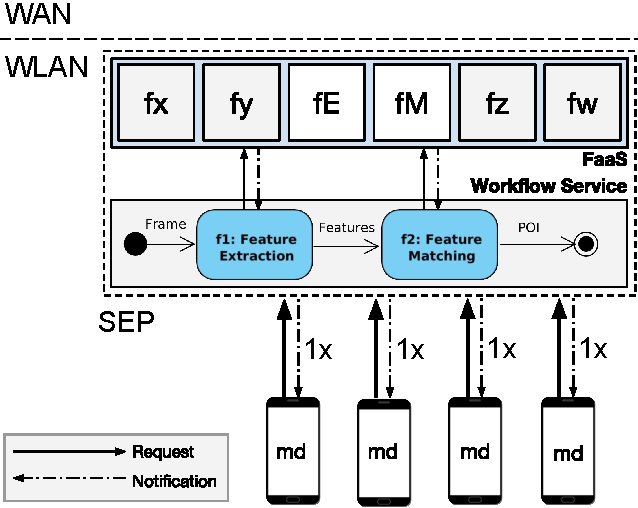
\includegraphics[width=1\linewidth]{Figs/Mobile_Computation_Offloading_Workflow.pdf}
	\caption{A workflow involving the sequential execution of the \textit{feature extraction} (fE) and \textit{matching} (fM) functions; each video frame generates a single (1x) request, which is sequentially processed by one instance of each function.} 
	\label{fig:Mobile_Computation_Offloading_Workflow}
\end{figure}

In a N-tier fog deployment~\cite{OpenFog:RA:2017}, latency-sensitive and data-intensive functions are best candidates for been placed in close proximity to the edge (e.g., SEPs co-located with 5G base stations~\cite{ETSI:MEC:2016:03}), whereas compute-intensive functions may require more powerful resources from intermediary fog nodes. Surrogate SEPs can also exploit \textit{east/west}~\cite{OpenFog:RA:2017} communication to maximize the availability of functions.

%As an example, 
Figure~\ref{fig:Mobile_Computation_Offloading_F1} depicts the two AR functions as a single service (1x request per offloading), whilst Figure~\ref{fig:Mobile_Computation_Offloading_F2} depicts each function as an independent service (2x requests per offloading). In the former, mobile devices (md) are unable to offload computation to SEP$_A$, as the fEM function is unavailable at that platform and the \textit{east/west} throughput is insufficient for delegating frequent requests with a video frame as payload. In the latter, data-intensive \textit{feature extraction} (fE) is provided by both SEPs, whilst \textit{feature matching} (fM) is unavailable at SEP$_A$. Requests targeting the fM function are delegated
to either SEP$_B$ (\textit{east/north}) or 
to the regional SEP$_R$ (\textit{south/north}),
%by its \textit{FaaS Controller},
%or to the cloud by a load balancer, 
thanks to the reduced payload size (\textit{video frame features}) and the low latency among these platforms. 



%TODO: change this figure for a sequence diagram
\begin{figure}[!bp]
	\centering
	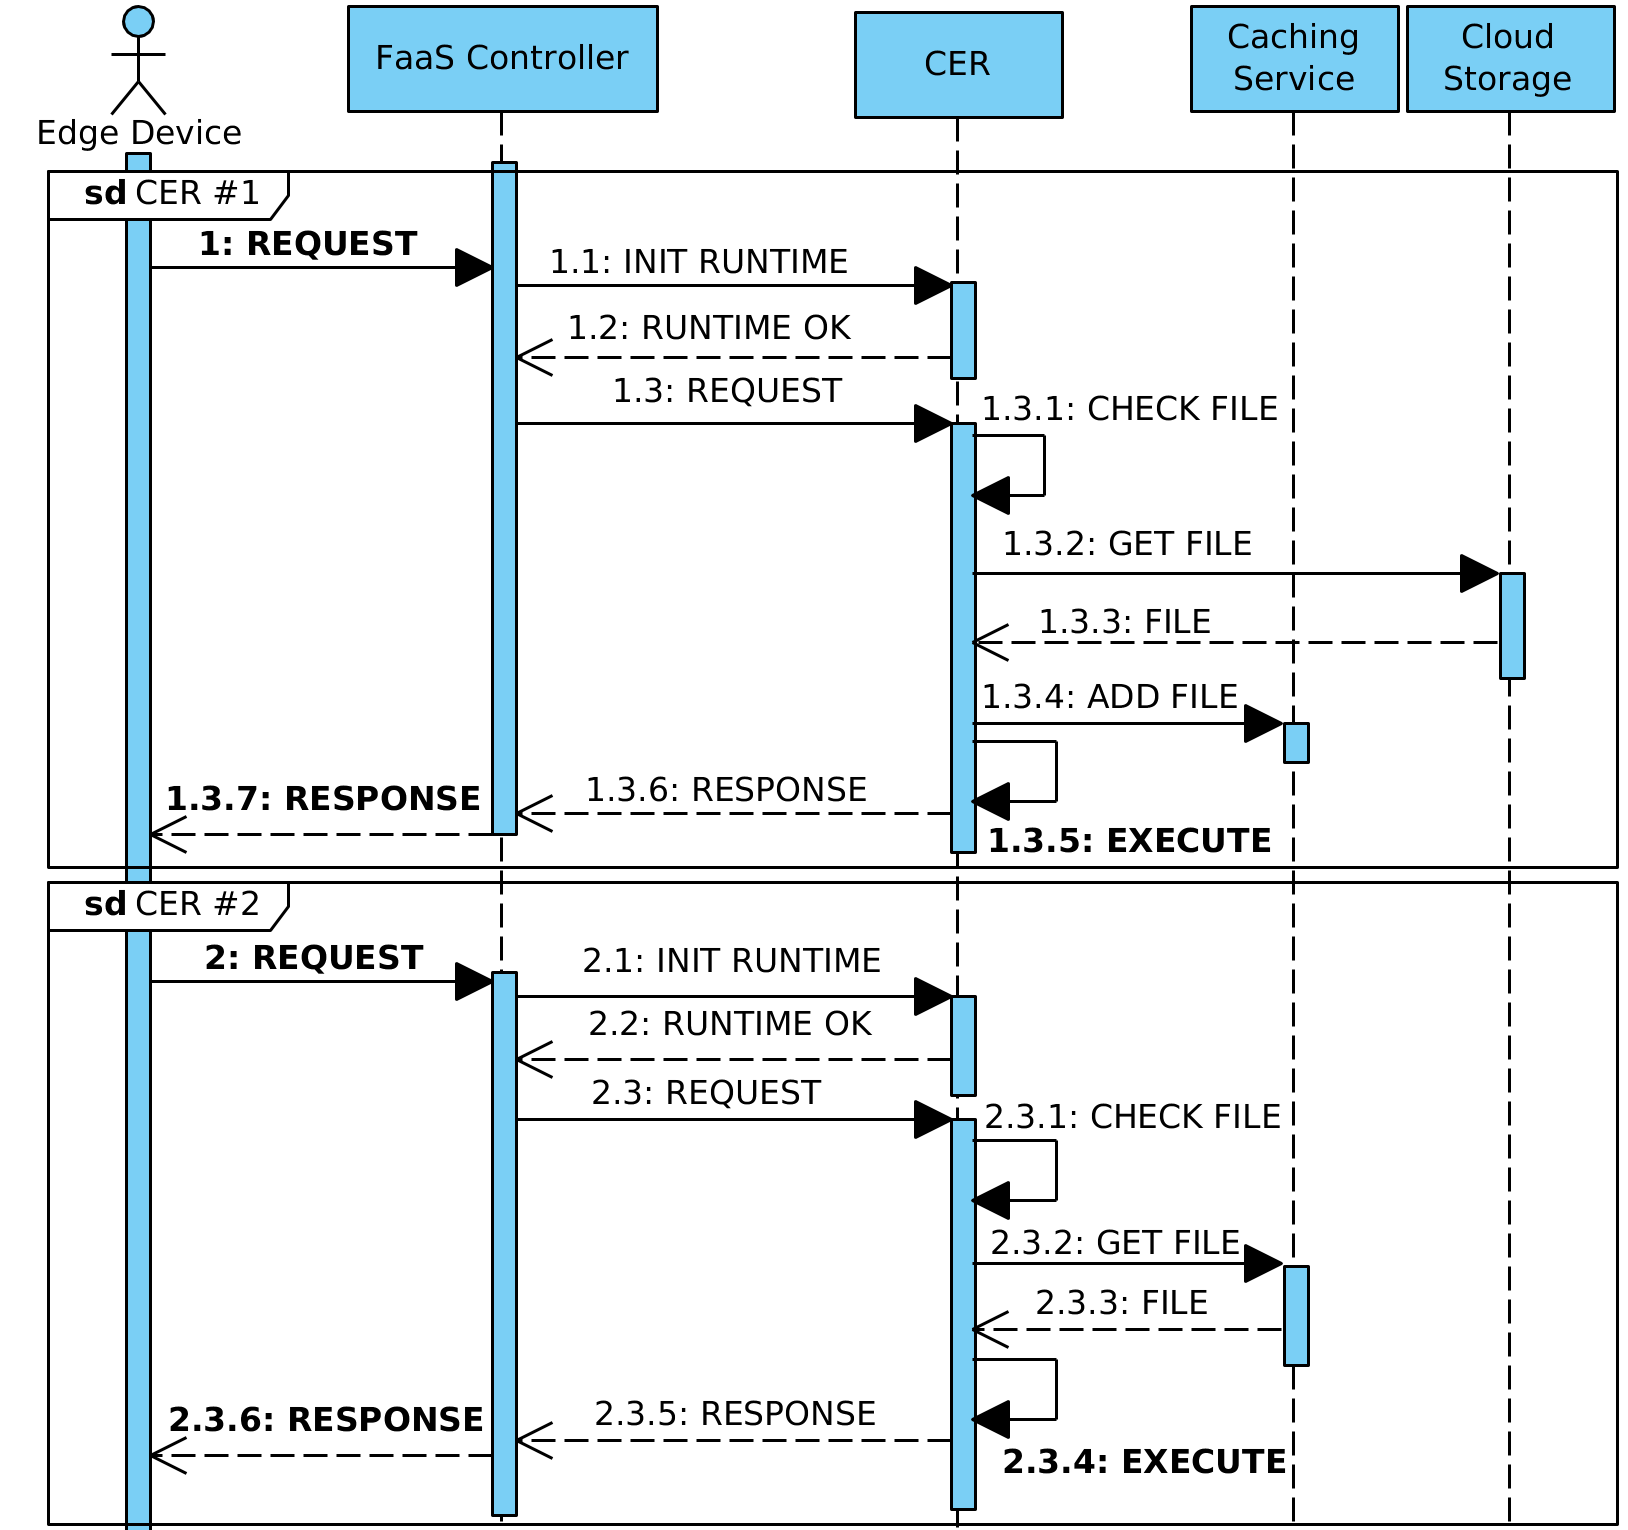
\includegraphics[width=1\linewidth]{Figs/CachingService}
	\caption{The very first function invocation fetches the file from a cloud storage and adds it to the \textit{Caching Service} for subsequent use by other CERs.} 
	\label{fig:Mobile_Computation_Offloading_Caching}
\end{figure}

%A SEP with three instances of the \textit{feature extraction} (fE) and two instances of the \textit{feature matching} (fM) functions; a copy of the POI catalog (PC) used by fM instances is fetched once from a cloud storage service

\subsubsection{Resource Management}
The FaaS model promotes efficiency by allocating resources in a timely and reactive manner. Notwithstanding this, inter-platform cooperation is paramount for increasing the scalability and robustness of provided services. 
From a centralized viewpoint, the orchestration of multiple SEPs faces many challenges: fine-grained functions demand fine-grained decisions on which platform they are executed; while part of the solution space can be filtered out at design time (e.g., based on capabilities and requirements), others should be performed at runtime in a timely manner to cope with client mobility and workload variations.
%In contrast with IaaS-based approaches, the actual CER instantiation is purely reactive; the placement decision delimits the share of resources allocated for each function in case of contention.
%In the AR example,

That considered,
we envision SEPs as self-contained entities able to cooperate in the automated provisioning and allocation of their resources. 
%needed to cope with distinct requirements and varying workloads. 
%The coordination space is limited by latency and throughput, 
%hence 
As latency and throughput are first class requirements,
SEPs cooperate
%(through its \textit{Controller}) 
with surrogate platforms within a latency/throughput threshold. For this, each platform advertises its capabilities, including the catalog of functions it supports. Additionally, they keep mutual information about the latency and throughput among them. Upon saturation, part of requests is delegated to the surrogate platform(s) best satisfying latency and throughput requirements, prioritizing those that are less frequently delegating requests of their own.

%While the specific details are out of the scope of this work, Section~\ref{sec:SEP_EDA} extends the discussion on the placement of functions and the balancing of the workload among SEPs.

%Its materialization would elevate the concept of serverless computing to the geographical level.

%Its materialization demands each SEP \textit{Controller}
%More details on the placement of functions and balancing of the workload are disucussed in Section~\ref{sec:SEP_EDA}.

%First, the FaaS model is based on events; 




%\subsubsection{Optimizations}







%\noindent
%\textbf{Optimizations:}
\subsubsection{Optimizations}
Notwithstanding the benefits of the FaaS model,
%in the provisioning of computing services, 
the satisfaction of low-latency requirements by a \textit{Serverless Edge Platform} demands further optimizations.

%In the FaaS model
First, functions are externally triggered by HTTP requests. In the context of real-time applications, communication overhead must be kept minimal. As such, the edge platform must include an interface that allows clients to trigger sequential or parallel execution of functions composing different services without the overhead associated to the HTTP protocol. For instance, the \textit{WebSocket protocol}
%\footnote{Documentation available at https://tools.ietf.org/html/rfc6455}
%is a standardized protocol that 
provides full-duplex communication channels over a single TCP connection. %Figure~\ref illustrates this feature.

%For this, each task is deployed as a stateless, fully-managed function and exposed as a web service. 
%Within milliseconds, the fully-managed platform allocates a containerized runtime instance in which the function is first executed, whereas subsequent executions may take advantage of existing instances.
%Dependencies, if any, are described within a package descriptor and made available by the platform.
%Finally, a third function gets detailed information about each POI from a remote database.
%In particular, OpenWhisk is an state-of-art and open source FaaS platform.

The support of an efficient protocol would enable real-time communication between edge devices and platforms. Still, individual function invocation may add significant latency overhead whenever two or more functions form an execution flow. To avoid this overhead, developers would be forced to either chain function calls through hardcoded dependencies, or write coarser and less cohesive functions. In the former case, the chaining of function also imposes a cost overhead, since caller functions are kept waiting.% for other function(s) to return. 

To address latency, design, cost, and resource efficiency concerns, we propose SEPs to be equipped with a \textit{Workflow Service}. This service allows developers to define, through visual or textual programming, a function execution flow.
%starting with the processing of the input sent by a client and finishing with the result sent back to the client. 
Similarly to single functions, workflows are triggered by events (e.g., an external request); at each intermediary step, result from the current function is passed to the next one. 

\begin{figure}[bp]
	\centering
	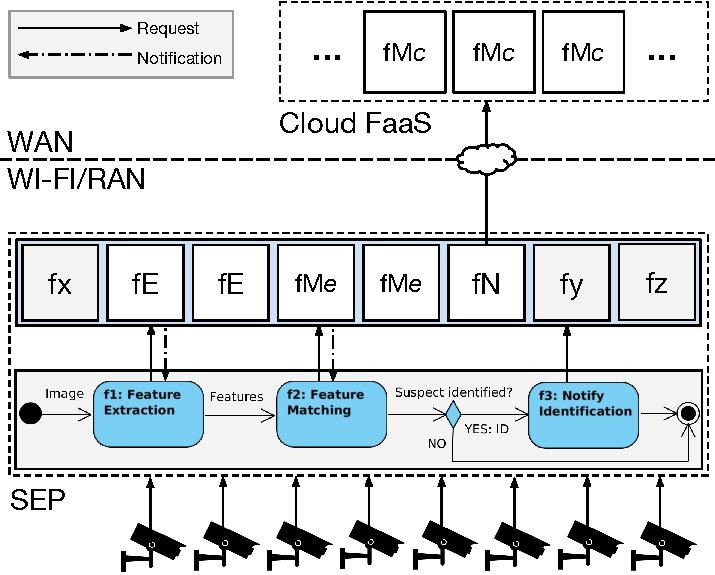
\includegraphics[width=\linewidth]{Figs/Edge_Data_Analytics_Video_Surveillance.pdf}
	\caption{Features from video frames captures by IoT cameras are \textit{extracted} (fE) and, upon positive \textit{matching} (fM$e$), sent for further analysis by a cloud service (fM$c$).}
	\label{fig:Edge_Data_Analytics_Video_Surveillance}
\end{figure}

\begin{figure}[bp]
	\centering
	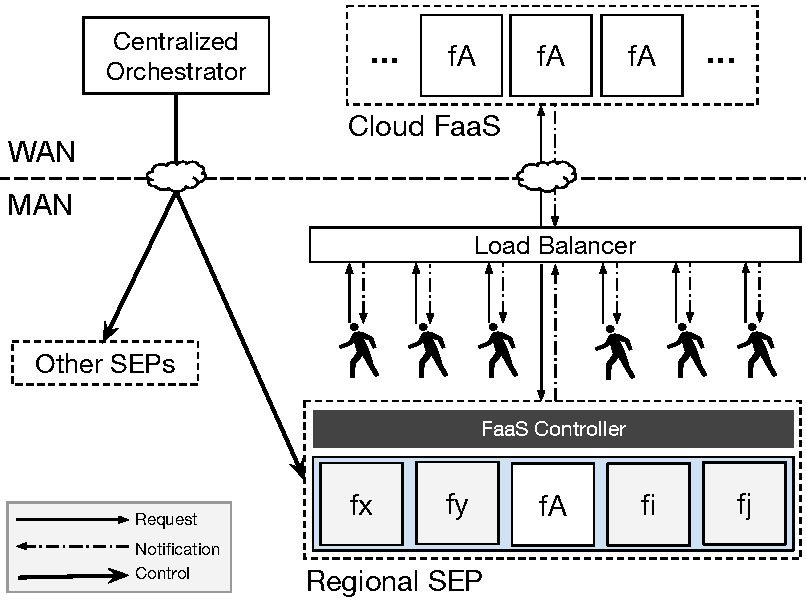
\includegraphics[width=\linewidth]{Figs/Edge_Data_Analytics_Personal_Assistant.pdf}
	\caption{Nº of instances of the \textit{health analysis} function (fA) hosted by a Regional SEP is limited by a \textit{Centralized Orchestrator}; given the number of allocated instances, the latency requirements and the average response time, a \textit{Load Balancer} distributes requests among the SEP and the cloud-based FaaS.}
	\label{fig:Edge_Data_Analytics_Personal_Assistant}
\end{figure}

Going back to the AR example, Figure~\ref{fig:Mobile_Computation_Offloading_Workflow} depicts a simple workflow consisting of the sequential execution of the \textit{feature extraction} and \textit{matching} functions, which remain decoupled. In contrast with Figure~\ref{fig:Mobile_Computation_Offloading_F2}, both functions are served by the same SEP. A similar inter-platform cooperation could still be achieved with the delegation of requests coming from the \textit{Workflow Service} at one SEP to surrogate SEPs.

Last but not least, existing FaaS platforms (e.g., AWS Lambda~\cite{AWSLambda} and Apache OpenWhisk~\cite{OpenWhisk}) enforce a programming model in which functions have access to a transient container folder without guaranteeing that subsequent invocations will be handled by the same CER. %Thus, each invocation must check whether cached data is available. 
In the context of latency-sensitive applications, retrieving extensive data sets may add prohibitive overhead. For instance, in the AR example, a catalog (circa 1Gb) is used in the identification of points of interest (POI).
% against their matched features. 
Due to size limitations, it can not be packed with the function source code, but needs to be retrieved dynamically by each new CER instance.
%Cloud vendors provide storage services as part of their platform ecosystem. 

%TODO: make it consistent with the PROTOTYPE Section
%To address the need of edge services with dependency to large data sets
Addressing the aforementioned concern, we propose to equip SEPs with a \textit{Caching Service}. This service allows SEP functions to fetch data from the cloud and keep it available at the edge for mitigating networking overhead. 
%More precisely, the \textit{Caching Service} would consist of an object-based storage system (e.g., AWS S3), in which files are associated with metadata.  

%To make use of this service, SEP functions post a file passing its cloud \textit{URI}.
% which should return a valid file format.
% --- and an optional expiration policy. 
%The file is then stored along with metadata containing both its URI and the frequency of access. %subsequent requests are served with minimum overhead. 


The diagram in Figure~\ref{fig:Mobile_Computation_Offloading_Caching} depicts the interplay between a CER instance initialized with the \textit{feature matching} (fM) function and the \textit{Caching Service}.
Upon a first invocation, the fM function fetches a POI catalog (PC) from a cloud storage and adds it to the \textit{Caching Service} passing its cloud \textit{URI}. 
The file is then stored along with metadata containing both its URI and the frequency of access.
%and to its CER transient folder. 
Subsequent invocations handled by other CERs retrieve the cached file with a single request.
To cope with the limitation of storage resources, cached files are rotated according to their access frequency. %As such, files accessed less frequently are subject for been replaced in case of resource contention. 
%%Files without an expiration date are replaced only in case of resource contention following the access frequency policy. 


\begin{figure*}[bh]
	\centering
	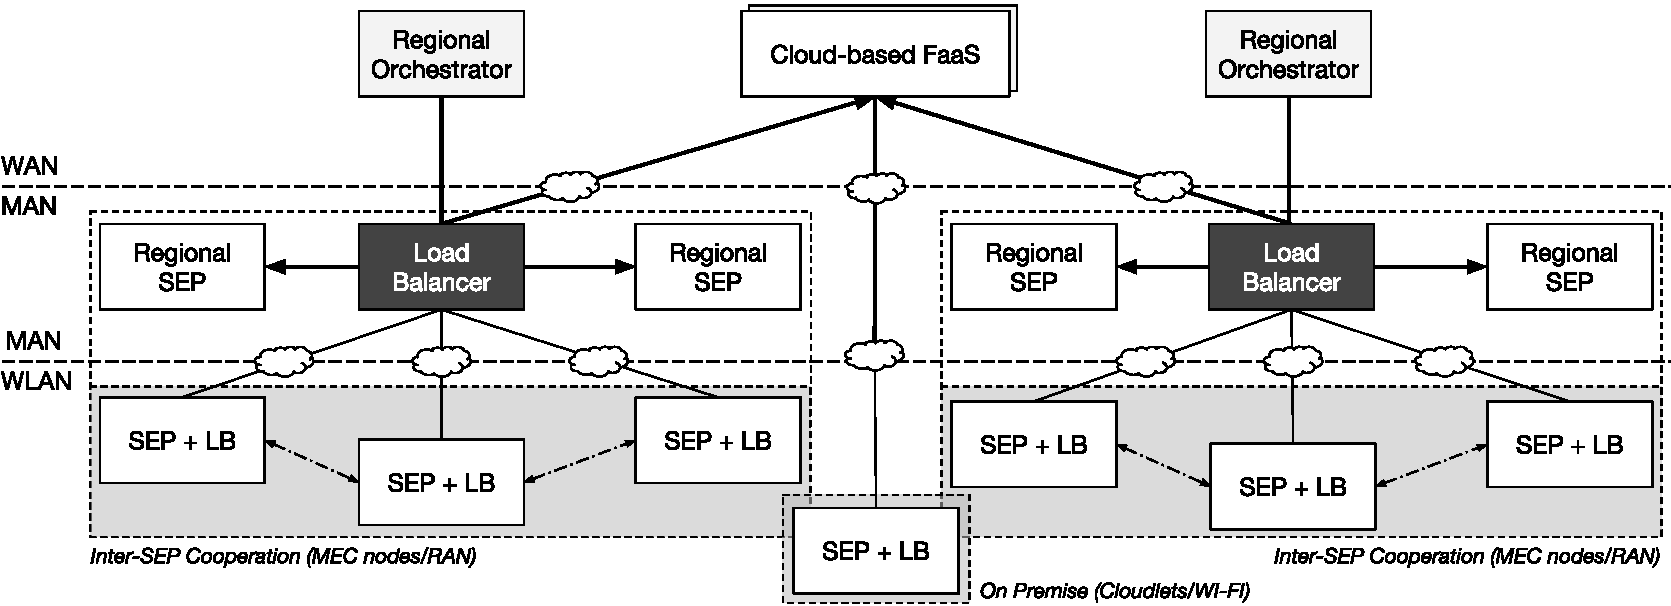
\includegraphics[width=1\linewidth]{Figs/Edge_Load_Placement_Expanded}
	\caption{Distribution of the workload for distinct functions among local SEPs, regional SEPs, and cloud-based FaaS platforms by hierarchical load balancers.}
	\label{fig:Edge_Load_Placement}
\end{figure*}

%A serverless edge platform should support a more efficient caching service to optimize use cases in which functions have data dependencies. 
\subsection{Edge Data Analysis}\label{sec:SEP_EDA}

The advent of data-intensive applications empowered by mobile and IoT devices raises concerns about the feasibility of sending exponentially larger volumes of data through the Internet all the way to cloud data centres. Accordingly, another important motivation for edge computing consists of the anticipation of the analysis of data produced and consumed by applications at the network edge. 

%TODO: find an example with low-latency requirement?
%Differently from the mobile computation offloading scenario, the most important concerns of edge data analysis are network throughput 
%(to cope with large volumes of data) 
%and preventing network bottlenecks caused by centralization. Still, edge analysis may also need to cope with low-latency requirements, specially if analysis results should feed latency-sensitive actuation.


%To illustrate this scenario
For example, in the context of smart cities and cyber-physical-systems, let us consider a video surveillance application 
depicted in Figure~\ref{fig:Edge_Data_Analytics_Video_Surveillance}. Similarly to the AR application, compute-intensive functions such as \textit{feature extraction} (fE) and \textit{matching} (fM\textit{e}) are assigned to  SEPs.
%, this time with the purpose of recognizing faces from a police catalog. 
These functions compose a workflow exposed as a service and consumed by resource-constrained IoT cameras; video frames are received at short intervals, from which facial features are extracted and matched against a police catalog (PC). A positive identification triggers the execution of a cloud-based service (fM\textit{c}) responsible for a more robust analysis able to detect false positives. In this manner, large volumes of data are processed at the edge, preventing the congestion of the wide area network (WAN) and centralized cloud services.


Still in the context of edge data analysis, 
%other use cases exhibit more strict requirements for latency. For instance, 
let us imagine that in the future the majority of elderly people will wear body sensors to collect data about their health status. In the event of an emergency (e.g., the beginning of a heart attack), emergency services should be dispatched immediately to the person location. Also, it is very important to provide the user with feedback so she can ask for support from other people.
%other people that can provide a first and immediate assistance.
%The IoT-based heart disease monitoring system for pervasive healthcare service
The accurate identification of such events, however, requires a complex analysis of data from different sensors (e.g., heart rate, oxigen saturation, glucose)~\cite{Li:2017}. Offloading the analysis from all users to the cloud may add substantial load to the WAN and centralized cloud services. %Instead, this burden should be shared with SEPs.% composing the mobile networks infrastructure (e.g., base stations, multi-technology aggregation sites, etc~\cite{}). 

 

%\subsubsection{Deployment}

The aforementioned examples share one characteristic: their main purpose is to prevent large volumes of data to be sent and processed by distant data centres. In the latter example, providing feedback in a timely manner is important, but does not fall into the low ($\leq 100ms$) or ultra-low ($\leq 20ms$) latency categories. For this kind of application and in contrast with the scenario in Section~\ref{sec:SEP_MCO}, functions are offloaded from cloud data centres to SEPs; also, the resulting placement decision is \textit{opportunistic} and informed by the availability of computing and networking resources, as well as the characteristics and requirements of each function. 

%TODO
Notice that, coherently with the FaaS model, the actual CER instantiation is purely reactive; the placement decision delimits the share of resources available for each function in case of contention.
Its ultimate goal is to optimize the allocation of SEP resources, considering the \textit{utility} of each function (e.g. in mitigating WAN congestion). As it requires a broader view of the system, placement is orchestrated in a centralized or hierarchical manner, accordingly to the fog architecture~\cite{Mach:2017}.  


%\subsubsection{Resource Management}

%As discussed in Section~\ref{sec:SEP_MCO}, the proposed architecture (see Figure~\ref{fig:Mobile_Computation_Offloading}) enables fine-grained functions to be placed onto different platforms. %In addition to SEPs, delay-tolerant functions can be also deployed to cloud-based FaaS platforms. 
%Liu:2014,K.Wang:2015
%

%The placement decision can be orchestrated in a centralized, hierarchical, or decentralized manner~\cite{Mach:2017}.  

%TODO SDN only or VNF? LB placement: where and why
For a given a placement decision, informed \textit{load balancers} make the timely decision on the destination of each request, taking into account the average response time and latency requirements. 
To render this decision transparent to end-users, 
load balancers are a constituent part of the SEP architecture or the network infrastructure itself. 
While this configuration is suitable to SEPs in close proximity with end-users (e.g., co-located with WLAN or RAN infrastructures), it may add substantial latency if the SEP lies many network hops away from the natural path to the cloud alternative. In this case, external load balancers should anticipate request distribution among regional SEPs and cloud-based FaaS platforms.


%The materialization of such a dynamic network component can benefit from the concept of \textit{Software Defined Networks} (SDN), considered one of the enabling technologies for edge computing~\cite{Mach:2017}. 
%Finally, the decision of where to send requests can also involve the participation of client devices~\cite{Baresi:2018}.

% and the workload of centralized services). 





% arriving at each SEP.
%arriving at its own SEP.


%load balancers to be dynamically created and managed to reflect the dynamicity of Internet applications. 
%Figure~\ref{} illustrates an hierarchical architecture composed of SDN-based Load Balancers.



%Differently from the mobile computation offloading scenario, edge data analysis may tolerate higher delays, in which case a \textit{scheduler} should decide between edge-based and cloud-based services. 

Figure~\ref{fig:Edge_Data_Analytics_Personal_Assistant} illustrates the opportunistic placement of a \textit{health analysis} function (fA) onto a Regional SEP. Based on the workload and the availability of computational and network resources, a \textit{Centralized Orchestrator} decides for the \textit{maximum number} of CER instances the SEP can host for each function.
%,  and informs this decision to the \textit{Load Balancer}. 
New CER instances are allocated on demand, accordingly to the FaaS model. As the volume of requests grows and the limited is achieved, response time increases and part of the requests are diverged
by the external \textit{Load Balancer} to a cloud-based FaaS.
%
%Still in Figure~\ref{fig:Edge_Data_Analytics_Personal_Assistant} example, 
Upon an emergency, function fA proceeds with two actions: i) the invocation of an 
%external 
%TODO reverse proxy x geographical DNS
\textit{Emergency Service}; and ii) the notification of the corresponding \textit{personal assistant device}. For this, the \textit{Load Balancer} works as a \textit{reverse proxy} to assure results will be sent back to devices regardless of the platform each request has been assigned to.

Concluding this section, Figure~\ref{fig:Edge_Load_Placement} presents the distribution of the workload by co-located and external load balancers (LB). Computation offloading and data analysis functions with stringent requirements for latency and throughput are served by local SEPs accessible through RAN or WI-FI;
other latency-sensitive and data-intensive functions are served by regional SEPs covering a metropolitan network area (MAN); 
remaining workload, including data analysis extrapolating edge capabilities, is served by cloud-based FaaS platforms. 





%In particular, the scheduling should take into account the latency constraints of each type of service.

%For instance, let us consider the case of a mobile crowd sensing application in which environmental data (e.g., air pollution~\footnote{a common type of sensor in smartphones in China}) is collected from sensors embedded in smartphones, tablets, and variables accompanying people. 

%This example poses one challenge: if functions are stateless and their instances ephemeral, how should the platform deal with long-living cases of data analysis? 

\subsection{Real-time Edge Coordination}\label{sec:SEP_RTEC}

\begin{figure}[bp]
	\centering
	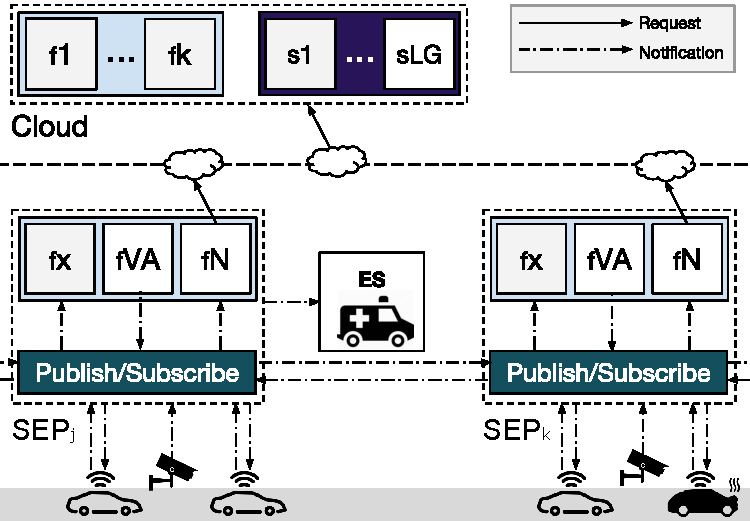
\includegraphics[width=1\linewidth]{Figs/Edge_Coordination_AVs_wide.pdf}
	\caption{Autonomous Vehicles, a road monitoring system, an emergency service and a logging service are coordinated by means of a distributed event bus hosted by surrogate SEPs.}
	\label{fig:Edge_Coordination_AVs}
\end{figure}

Another important edge application scenario involves the coordination among distributed mobile and IoT devices. %at the network edge. 
To illustrate this scenario, let us consider the coordination among \textit{Autonomous Vehicles} (AV). %Each vehicle is expected to generate large volumes of data from its sensors, including the AV's actual position, speed, and acceleration. 
AVs make use of sophisticate mechanisms to prevent collisions. Notwithstanding this, AVs traveling at high speeds would benefit from real-time notification of anomalous events in their path. 

Addressing this scenario, SEPs feature a \textit{Publish-Subscribe Service (Pub-Sub Service)}. This service allows edge devices (e.g., AVs, monitoring cameras) and additional edge-based systems (e.g., a road monitoring system) to coordinate through events.
%integrated with the edge platform. 
%(e.g., among AVs connected to different SEPs). 
Other systems (e.g., an emergency service) can also subscribe to specific events in order to take timely actions (e.g., to dispatch ambulances or road patrols).

In addition to localized coordination, surrogate SEPs (e.g., at different road sections) form a distributed event bus enabling inter-platform coordination. Moreover, in the context of IoT, a \textit{Pub-Sub Service} must take into account the specific protocols used by edge devices. For instance, many IoT devices make use of MQTT, a \textit{Machine to Machine} (M2M) pub-sub protocol. 

The integration enabled by a \textit{Pub-Sub Service} fits well in a serverless architecture~\cite{Lloyd18serverless}. Not only the FaaS model enforces an event-driven architecture by design, but existing platforms (e.g., AWS Lambda~\cite{AWSLambda}) also integrate with other services through asynchronous, event-based notification services (e.g., AWS \textit{Simple Notification Service}). 

%Indeed, existing FaaS platforms (e.g., AWS Lambda~\cite{AWSLambda}) are integrated with other systems by means of pub-sub services (e.g., AWS SNS) in which functions are triggered by event notifications. 

%In the AV coordination example, the \textit{Pub-Sub Service }
%could be used to trigger, upon an anomalous event, 
%enables the triggering of a specific SEP function responsible for the invocation of an external service (e.g., a cloud-based service that logs the occurrence of the anomalous event). 

Figure~\ref{fig:Edge_Coordination_AVs} illustrates the solution for AVs coordination. Each AV subscribes to a surrogate SEP deployed to roadside units (RSU) integrated with video surveillance cameras (VSC); anomalous events --- published by AVs or by \textit{video analysis} functions (fVA) --- are propagated to the AVs connected to the SEP of origin, to those behind, and to the nearest emergency squad (ES). Finally, a cloud-based logging service (sLG) is invoked by a notification function (fN), triggered by same event. To prevent multiple invocations, the notification function at each SEP must distinguish between local events and those from other platforms. The same is valid for the emergency squads covering different road sections. To satisfy this requirement, the \textit{Pub-Sub Service} enforces location-awareness by mapping each event to its SEP of origin.

\subsection{Stateful Edge Services}

\begin{figure}[bp]
	\centering
	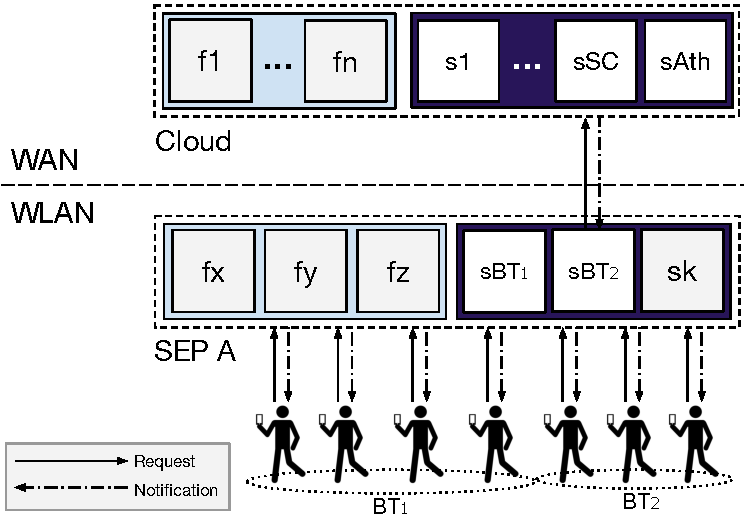
\includegraphics[width=1\linewidth]{Figs/Stateful_Edge_Services.pdf}
	\caption{A stateful service enables players to join MMG battle sessions (BT$_1$, BT$_2$); instances (sBT$_1$, sBT$_2$) are mapped to each session; authentication (sAuth) and player scores (sSC) are managed by cloud-based services.}
	\label{fig:Steteful_Edge_MMG}
\end{figure}

One of the most important directives concerning the design of web services is to move state into a separate layer~\cite{Armbrust:2010}. Stateless services are easier to test, debug, and scale, whereas stateful services require state to be recreated for testing and debug purposes. Moreover, achieving consistency among replicated instances incur in performance degradation. The FaaS model embraces this directive with stateless functions.
%, suitable for the application scenarios discussed in the previous sections. 
However, some types of applications exhibit particular needs that justify the adoption of stateful services by a SEP.

%To illustrate this requirement, 
For example, let us think of a mobile multiplayer game (MMG). As an interactive application, low-latency is a first class requirement that justifies the deployment of services to the network edge. In this category, \textit{PokemonGO} is 
a MMG featuring a single interactive use case in which players interact with \textit{Pokemons}, a virtual creature collected by players.
% added to their devices screen. 
To increase the game popularity, we conceive a new feature to enables users in the same city area to start game battles involving their \textit{Pokemons}. 

Following a conventional multi-player architecture, an authoritative service is designed to host the game battle state and logic. This solution has two advantages. First, it prevents the overhead of transferring to the service, at each user interaction, the whole state of the battle. Second, it allows an authoritative service to manage changes to the game state that may not be safely delegated to clients, who otherwise could modify the local game logic and state to their own advantage.

%In particular, the state represents a battle session, whilst business logic is responsible for updating the state according to user inputs and other events. 

To address this requirement, we propose to equip SEPs with a \textit{Stateful Service}. 
%However, the support for stateful services comes with a cost. 
%address the specific use cases requiring stateful services
To cope with the need of efficient allocation of resources, the \textit{Stateful Service} mimics the FaaS model. More precisely, stateful application partitions are designed to last for a limited duration corresponding to the lifetime of a specific latency-sensitive use case. Similarly to the FaaS model, stateful partitions are hosted by CERs created on demand in a timely manner. The main differences are:

\begin{itemize}
    
    \item CERs are initialized with a unique \textit{session token} upon an application specific event (e.g., the \textit{start of a battle});
    
    \item users within the same session (e.g., \textit{a battle}) share the same token, which is passed to the SEP at each request; %(e.g., a battle action); and
    
    \item requests are delegated to the corresponding CER instance, which is terminated upon application specific events (e.g., the \textit{end of a battle}).
    
\end{itemize}

%As with FaaS, 
The resulting model benefits from the container technology to provide stateful services without preallocating platform resources. 
%The main disadvantage lies on the scalability. In this regard, 
To prevent the consistency overhead that would arise with the synchronization of state along replicated instances, the allocation mechanism should privilege vertical scaling with the dynamic allocation of CPU and memory to the single CER instance hosting a stateful service. 

%Another challenge posed by stateful services is mobility. To tackle this problem, SEPs can either enforce that sessions are bind the CER to its SEP of origin



Figure~\ref{fig:Steteful_Edge_MMG} presents the game example. Users joining battles (BT$_1$ and BT$_2$) are identified by a common token, which is mapped to a specific CER instance (sBT$_1$ and sBT$_2$, respectivelly).
%(e.g., in a P2P architecture)
Composing the rest of the application, other delay-tolerant features (e.g., players scores) are managed by resourceful, long-living cloud-based services, accessed without SEP inter-mediation.  %Figure~\ref{fig:Steteful_Edge_MMG} depicts the resulting architecture.%; instances of the stateful \textit{multiplayer battle service} are hosted by the serverless edge platform precisely when needed. 

